\providecommand{\main}{../main}
\documentclass[\main/main.tex]{subfiles}
\graphicspath{{../images/}}
\begin{document}
\section{
    共形ブートストラップ
}
この章では共形ブートストラップについて概略を説明する。
技術的な部分については\cite{simmonsduffin2016tasi},\cite{Nakayama_2019}を参照してほしい。

この方法はモデルの具体的なHamiltonianを指定せずに、演算子積展開から導かれる相関関数の自己無撞着性によって、共形データを決定する試みである。
% 共形データが分かれば相関関数を再構成することができるので、共形ブートストラップは共形不変性だけから理論を解く試みだと言える。

\subsection{
    交差対称性(crossing symmetry)
}
相関関数を演算子積展開によって計算する時、演算子積展開を適用する順序には任意性がある。
異なる順序の計算は全て同じ結果を与えなければならない。
この条件を\textbf{交差対称性(crossing symmetry)}と呼ぶ。

まず、3点関数の交差対称性
\begin{align}
    𝒪₁⋅(𝒪₂⋅𝒪₃) = 𝒪₁⋅(𝒪₃⋅𝒪₂) = 𝒪₂⋅(𝒪₁⋅𝒪₃) = ⋯
\end{align}
から、演算子積展開の係数$f_{ijk}$に対して、
\begin{align}
    f_{ijk} = f_{ikj} = f_{jik}
\end{align}
が成り立つ。
つまり$f_{ijk}$は完全対称である。
これは$𝒪_i$が期待値の中で可換なことから自明な関係式である。

次に、4点関数の交差対称性を考える。
3点関数と4点関数についての交差対称性から、任意の$n$点関数についての交差対称性が導かれるので、これ以上の条件は必要ない。
簡単のために同一スカラープライマリー場の4点関数$\⟨ϕ(x₁)ϕ(x₂)ϕ(x₃)ϕ(x₄)\⟩$を考え、以下の2つの順序で計算する。
\begin{align}
    \⟨(ϕ(x₁)⋅ϕ(x₂))⋅(ϕ(x₃)⋅ϕ(x₄))\⟩
    = \⟨(ϕ(x₁)⋅ϕ(x₄))⋅(ϕ(x₂)⋅ϕ(x₃))\⟩
\end{align}
% \footnote{
%     演算子積展開の収束半径の問題を考える必要があるが、体積が有限の領域で2通りの計算がどちらも収束する。
    % 具体的には$ϕ(x₁),ϕ(x₂)$のみを含む超球と$ϕ(x₁),ϕ(x₄)$のみを含む超球があれば良いが、これらを達成する$x₁,x₂,x₃,x₄$は体積が有限の領域を成す。
% }
共形ブロックを用いると、4点関数は
\begin{align}
    ⟨(ϕ(x₁)⋅ϕ(x₂))⋅(ϕ(x₃)⋅ϕ(x₄))⟩
    = \÷{g(u,v)}{x_{12}^{2Δ_ϕ}x_{34}^{2Δ_ϕ}},
    \␣
    g(u,v) = ∑_𝒪f_{ϕϕ𝒪}^2g_{Δ_𝒪,l_𝒪}(u,v)
\end{align}
と書けるので、交差対称性から
\begin{align}
    \÷{g(u,v)}{x_{12}^{2Δ_ϕ}x_{34}^{2Δ_ϕ}}
    = \÷{g(v,u)}{x_{23}^{2Δ_ϕ}x_{14}^{2Δ_ϕ}}
\end{align}
が得られる。
この式は以下のようなダイアグラムで表される。
\begin{figure}[H]
    \centering
    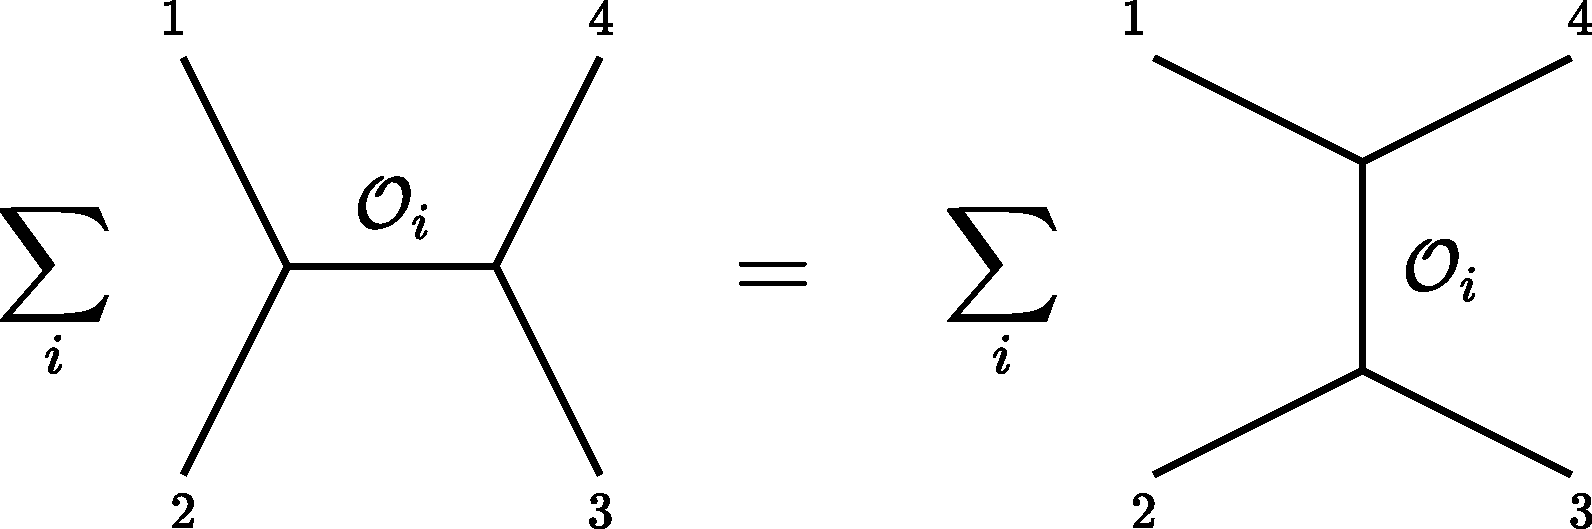
\includegraphics[width=0.5\hsize]{../images/OPE diagram.pdf}
    \caption{
        交差対称性を表すダイアグラム。
        左は$(ϕ(x₁)⋅ϕ(x₂))⋅(ϕ(x₃)⋅ϕ(x₄))$の順序で、右は$(ϕ(x₁)⋅ϕ(x₄))⋅(ϕ(x₂)⋅ϕ(x₃))$の順序で演算子積展開を適用することを表す。
    }
\end{figure}
また複比
\begin{align}
    u = z\=z = \÷{x_{12}^2x_{34}^2}{x_{13}^2x_{24}^2},
    \␣
    v = (1-z)(1-\=z)
    = \÷{x_{23}^2x_{14}^2}{x_{13}^2x_{24}^2}
\end{align}
を用いると、
\begin{align}
    v^{Δ_ϕ}g(u,v) = u^{Δ_ϕ}g(v,u)
\end{align}
が成り立つ。
これを共形ブロックを使って書くと、
\begin{align}\tcboxmath{
    ∑_𝒪 f_{ϕϕ𝒪}^2 F_{Δ_𝒪,l_𝒪}^{Δ_ϕ}(u,v) = 0,
    \␣
    F_{Δ,l}^{Δ_ϕ}(u,v)
    ≔\Q(
        v^{Δ_ϕ}g_{Δ,l}(u,v)
        -u^{Δ_ϕ}g_{Δ,l}(v,u)
    )
    \label{crossing equation}
}\end{align}
となる。
この式を\textbf{交差方程式(crossing equation)}と呼ぶ。
4点関数の交差対称性はもう一つあり、$x₁$と$x₂$を入れ替えることで
\begin{align}
    g(u,v) = g(u/v,1/v)
\end{align}
が成り立つ。
ただしこれは演算子積展開の順序交換$𝒪₁⋅𝒪₂ ↔ 𝒪₂⋅𝒪₁$についての対称性であり、自明な関係式である。
任意の置換に対する交差対称性は以上の2つの関係式から構成できる。

\subsection{
    共形データに対する制限
}
(\ref{crossing equation})は2変数の関数空間における無限次元の拘束条件となっている。
解析的に(\ref{crossing equation})から情報を引き出す試みもあるが、この節では厳密に解くことを諦め、不等式として共形データに対する制限を求めることにする。

まず、$f_{ϕϕ𝒪}^2 ≥ 0$に注目する。
\footnote{
    これを示すために実時間のシリンダー時空上での3点関数を考える。
    space-likeに離れた3点に対し、演算子が可換であることを用いると、
    \begin{align}
        ⟨0|ϕ₁(x₁)ϕ₂(x₂)𝒪^{μ₁⋯μₗ}(x₃)|0⟩^*
        = ⟨0|ϕ₁(x₁)ϕ₂(x₂)𝒪^{μ₁⋯μₗ}(x₃)|0⟩
    \end{align}
    となる。
    したがって$f_{ϕ₁ϕ₂𝒪}^* = f_{ϕ₁ϕ₂𝒪}$が言える。
    ただし場の演算子がHermite演算子であることを仮定した。
}
$p_{Δ,l} = f_{ϕϕ𝒪}^2$とおくと、(\ref{crossing equation})は
\begin{align}
    ∑_{Δ,l}p_{Δ,l}\→F_{Δ,l}^{Δ_ϕ} = 0,\␣
    p_{Δ,l} ≥ 0
    \label{crossing eq in vector space}
\end{align}
と書ける。
ここで$F_{Δ_𝒪,l_𝒪}^{Δ_ϕ}(u,v)$を$u,v$についての関数空間におけるベクトルとみなし、$\→F_{Δ_𝒪,l_𝒪}^{Δ_ϕ}$と書いた。
これは無限次元のベクトルだが、有限次元の部分空間に射映しても、以下の議論は問題なく成り立つ。

次に、演算子積展開に現れる$Δ,l$を仮定する。
つまり、$f_{ϕϕ𝒪}^2 > 0$となる$𝒪$の共形次元およびスピンを仮定する。
演算子積展開に現れる全ての$Δ,l$に対し、線型汎函数$α$で
\begin{align}
    α\Q(\→F_{Δ,l}^{Δ_ϕ}) ≥ 0
\end{align}
となるものがあったとしよう。
ただし、左辺が正になるような$Δ,l$が少なくとも1つ存在するとする。
このとき、
\begin{align}
    ∑_{Δ,l}p_{Δ,l}α\Q(\→F_{Δ,l}^{Δ_ϕ}) > 0
\end{align}
が成り立つ。
これは(\ref{crossing eq in vector space})と矛盾するので、仮定が排除される。
これによって、共形データに対する制限を課すことができる。

\cite{simmonsduffin2016tasi}にある具体例を紹介しよう。
2次元の共形場理論で、共形次元が$Δ_ϕ = 1/8$となるスカラープライマリー場$ϕ$を有する理論を考える。
$\→F$を以下の写像によって2次元の部分空間に射映する。
\begin{align}
    \→v(F)
    = \Q(
        H\Q(\÷{1}{2},\÷{3}{5})-H\Q(\÷{1}{2},\÷{1}{3}),
        H\Q(\÷{1}{2},\÷{3}{5})-H\Q(\÷{1}{3},\÷{1}{4})
    ) ∈ ℝ^2
\end{align}
ここで、
\begin{align}
    H(u, v) = \÷{F(u,v)}{u^{Δ_ϕ}-v^{Δ_ϕ}}
\end{align}
である。
% $\→v(F)$に対し、$p_{Δ,l} ≥ 0$が存在して
% \begin{align}
%     ∑_{Δ,l} p_{Δ,l}\→v(F) = 0
% \end{align}
% が成り立つ。
図\ref{fig: bootstrap in 2D subspace}は、ありうる全ての$l,Δ$に対し、$\→v(F_{Δ,l}^{Δ_ϕ})$をプロットしたものである。
\begin{figure}[H]
    \centering
    \includegraphics[width=0.6\hsize]{../images/bootstrap.png}
    \caption{
        \cite{simmonsduffin2016tasi}より引用。
        それぞれの軌跡はスピン$l$の演算子に対し、
        $Δ$を$Δ_\t{min} = l+d-2 = l$から始めて連続的に大きくしていった場合の$\→v(F_{Δ,l}^{Δ_ϕ})$を表す。
        $l$が奇数となる演算子はスカラー演算子の4点関数では現れないので無視している。
        この理由については\cite{simmonsduffin2016tasi}の9.4を参照してほしい。
    }
    \label{fig: bootstrap in 2D subspace}
\end{figure}
まず恒等演算子に対し、$F_{0,0}^{Δ_ϕ}(u,v)=u^{Δ_ϕ}-v^{Δ_ϕ}$となることから、$\→v(F_{0,0}^{Δ_ϕ})=(0,0)$となる。
また$l → ∞$としたとき、軌道は図の$y$軸に近づいていくことが読み取れる。

2次元空間を原点を通る直線で2つに分けた時、演算子積展開に現れる全ての演算子が片側に分布してしまうと、ベクトル$\→u$が存在して
\begin{align}
    α(F_{Δ,l}^{Δ_ϕ}) ≔ \→u⋅\→v(F_{Δ,l}^{Δ_ϕ}) > 0
\end{align}
となってしまう。このとき交差対称性を満たすことはできない。
ここでスピン$0$の演算子に注目すると、交差対称性を満たすためには$Δ ∈ [0.161,1.04]$となるような演算子が演算子積展開に現れなければならないことが分かる。

この制限がどこまで強いものなのかを、厳密解と比較して考えてみる。
2次元Ising模型は実スカラー場$σ$をもち、その共形次元は$Δ_σ=1/8$である。
$σ×σ$の演算子積展開に現れるもっとも次元の低いスカラー場はエネルギー演算子$ε$であり、その共形次元は$Δ_ε = 1$である。
つまり、$Δ_\t{scalar} ≤ 1.04$は実際の理論に対して4\%程度の精度で上限を与えていることが分かる。

以上で紹介したのはは2次元の部分空間での制限だが、より大きな部分空間で計算することで、より強い制限が期待できる。
一般には部分空間への射映を$z=\=z=1/2$まわりのTaylor展開
\footnote{
    $z=\bar{z}=1/2$は4点関数の計算における2つの演算子積展開の収束半径の共通部分に含まれる。
}
によって行い、$α(F)$を
\begin{align}
    α(F)
    = ∑_{m+n≤Λ} a_{mn}∂_z^m∂_{\=z}^nF(z,\=z)
    \E_{z=\=z=\÷{1}{2}}
\end{align}
と定義する。
ここで$Λ$は微分の次数に対するカットオフである。
このような部分空間に対し、$α(F) ≥ 0$となるような$α$が存在しないことから、演算子積展開に現れる演算子の共形次元に制限をつける。

これは人間の手に負えるものではなく、計算機を用いて実行される。
しかし、計算機をもってしても無限に大きいスピン・共形次元は計算できないので、どこかで計算の打ち切りが存在する。
ただし、共形ブロックとその$z=\=z=1/2$での微分は$l$が大きな極限ですばやく収束することが経験的に知られており、十分大きなスピンで打ち切れば結果に影響は出ない。
また共形次元$Δ$が無限大、あるいは連続的な値を取り得ることも問題であるが、いくつかの対処法がある\cite{simmonsduffin2016tasi}。

\subsection{
    3次元Ising模型への適用
}

いよいよ3次元Isingモデルへの適用を考えよう。
我々はまず、$ℤ_2$変換に対して$ϕ → -ϕ$となるようなスカラー場$ϕ$を考える。
演算子積展開$ϕ×ϕ$の中で、最も次元の小さいスカラー場の次元を$Δ_0$とする。
$ϕ×ϕ$は$ℤ_2$対称だから、$ϕ$は現れない。
ここで
\begin{align}
    α(F)
    = ∑_{m+n≤Λ} a_{mn}∂_z^m∂_{\=z}^nF(z,\=z)
    \E_{z=\=z=\÷{1}{2}} ≥ 0,\␣
    Δ ≥
    \begin{cases}
        Δ₀ & (l = 0),\\
        l+d-2 & (0 < l < l_\t{max})
    \end{cases}
\end{align}
となる線型汎函数$α(F)$を探す。この問題は半正定値計画法という問題に書き換えることができ、これについては数値的に効率よく解くアルゴリズムが存在する。
もし$α(F)$が存在したならば、$Δ₀$より小さい次元をもつスカラー演算子が存在しなければならない。
この$Δ₀$を2分探索しながら変化させていくことで、あり得る$Δ₀$の上限$Δ_0^\t{crit.}$を求めることができる。
以下は$ϕ$の次元$Δ_ϕ$を変化させながら、$Δ_0^\t{crit.}$をプロットしたものである。
\begin{figure}[H]
    \centering
    \begin{tabular}{cc}
        \begin{minipage}[b]{0.45\hsize}
            \includegraphics[width=\hsize]{../images/bootstrap_2dising.png}
        \end{minipage}
        &
        \begin{minipage}[b]{0.45\hsize}
            \includegraphics[width=\hsize]{../images/bootstrap_3dising.png}
        \end{minipage}
    \end{tabular}
    \caption{
        $ℤ₂$対称な2次元理論(左)と3次元理論(右)に対する共形ブートストラップ。
    }
\end{figure}
2次元Ising模型の厳密解は許される領域の端にある折れ曲がりの上にいる。
\footnote{
    また、2次元の他のミニマルモデルも領域の端にある。
    ミニマルモデルについては\cite{Hikita_2020}や\cite{francesco2012conformal}を参照してほしい。
}
3次元の場合も同様の振る舞いが見られ、折れ曲がり
\footnote{
    キンクと呼ばれる。
}
に3次元臨界Ising模型がいることが予想できる。
したがって、この折れ曲がりの位置を特定することで、3次元臨界Ising模型の共形次元を計算することができる!
また、relevantな演算子の共形次元から臨界指数を直ちに求めることができる。

ただ、これでは納得のいかない方もいるかもしれない。
折れ曲がりにIsing模型がいるというのは単なる推測である。
しかし、上の図はあくまで1つの4点関数についての計算であり、より多くの4点関数についての交差対称性を考えることで、領域を狭めることができる。
図\ref{boot_3dising}は、$\⟨σσσσ\⟩,\⟨σσεε\⟩,\⟨εεεε\⟩$という3種類の4点関数について共形ブートストラップを行った結果である。
さらにここではrelevant($Δ<d=3$)な演算子が$ℤ₂$対称なスカラー演算子と$ℤ₂$反対称なスカラー演算子の2種類であるという仮定を用いている。
これはIsing模型の相転移が温度($ℤ₂$対称)と磁場($ℤ₂$反対称)を調節しておこる相転移であることから従う性質である。
\begin{figure}[H]
    \centering
    \includegraphics[width=0.6\hsize]{../images/bootstrap_ising.png}
    \caption{
        \cite{simmonsduffin2016tasi}より引用。
        relevantな演算子が$ℤ₂$対称なスカラー演算子と$ℤ₂$反対称なスカラー演算子の2種類であると仮定し、
        $\⟨σσσσ\⟩,\⟨σσεε\⟩,\⟨εεεε\⟩$について共形ブートストラップを行った結果。
        $Λ=12$としている。
    }
    \label{boot_3dising}
\end{figure}
すると、先ほどは折れ曲がりだったところが島のように孤立している。
この領域の中に3次元臨界Ising模型は位置しており、微分の次数のカットオフ$Λ$を上げていくことで、島を狭めていくことができる。
図\ref{comparison}は$Λ=43$の計算についてモンテカルロ法との比較をした図であり、モンテカルロ法の精度を超えて共形次元が決定されることがわかる。
\begin{figure}[H]
    \centering
    \includegraphics[width=0.6\hsize]{../images/comparison.png}
    \caption{
        \cite{Kos_2016}より引用。モンテカルロ法による共形次元の計算(点線の枠)と$Λ = 43$での共形ブートストラップの計算(青枠)の比較。
    }
    \label{comparison}
\end{figure}
\end{document}